
\documentclass{exam}

\usepackage{units} 
\usepackage{graphicx}
\usepackage[fleqn]{amsmath}
\usepackage{cancel}
\usepackage{float}
\usepackage{mdwlist}
\usepackage{booktabs}
\usepackage{cancel}
\usepackage{polynom}
\usepackage{caption}
\usepackage{fullpage}
\usepackage{xfrac}
\usepackage{enumerate}

\newcommand{\degree}{\ensuremath{^\circ}} 
\everymath{\displaystyle}

% \begin{figure}[H]
%   \centering
%   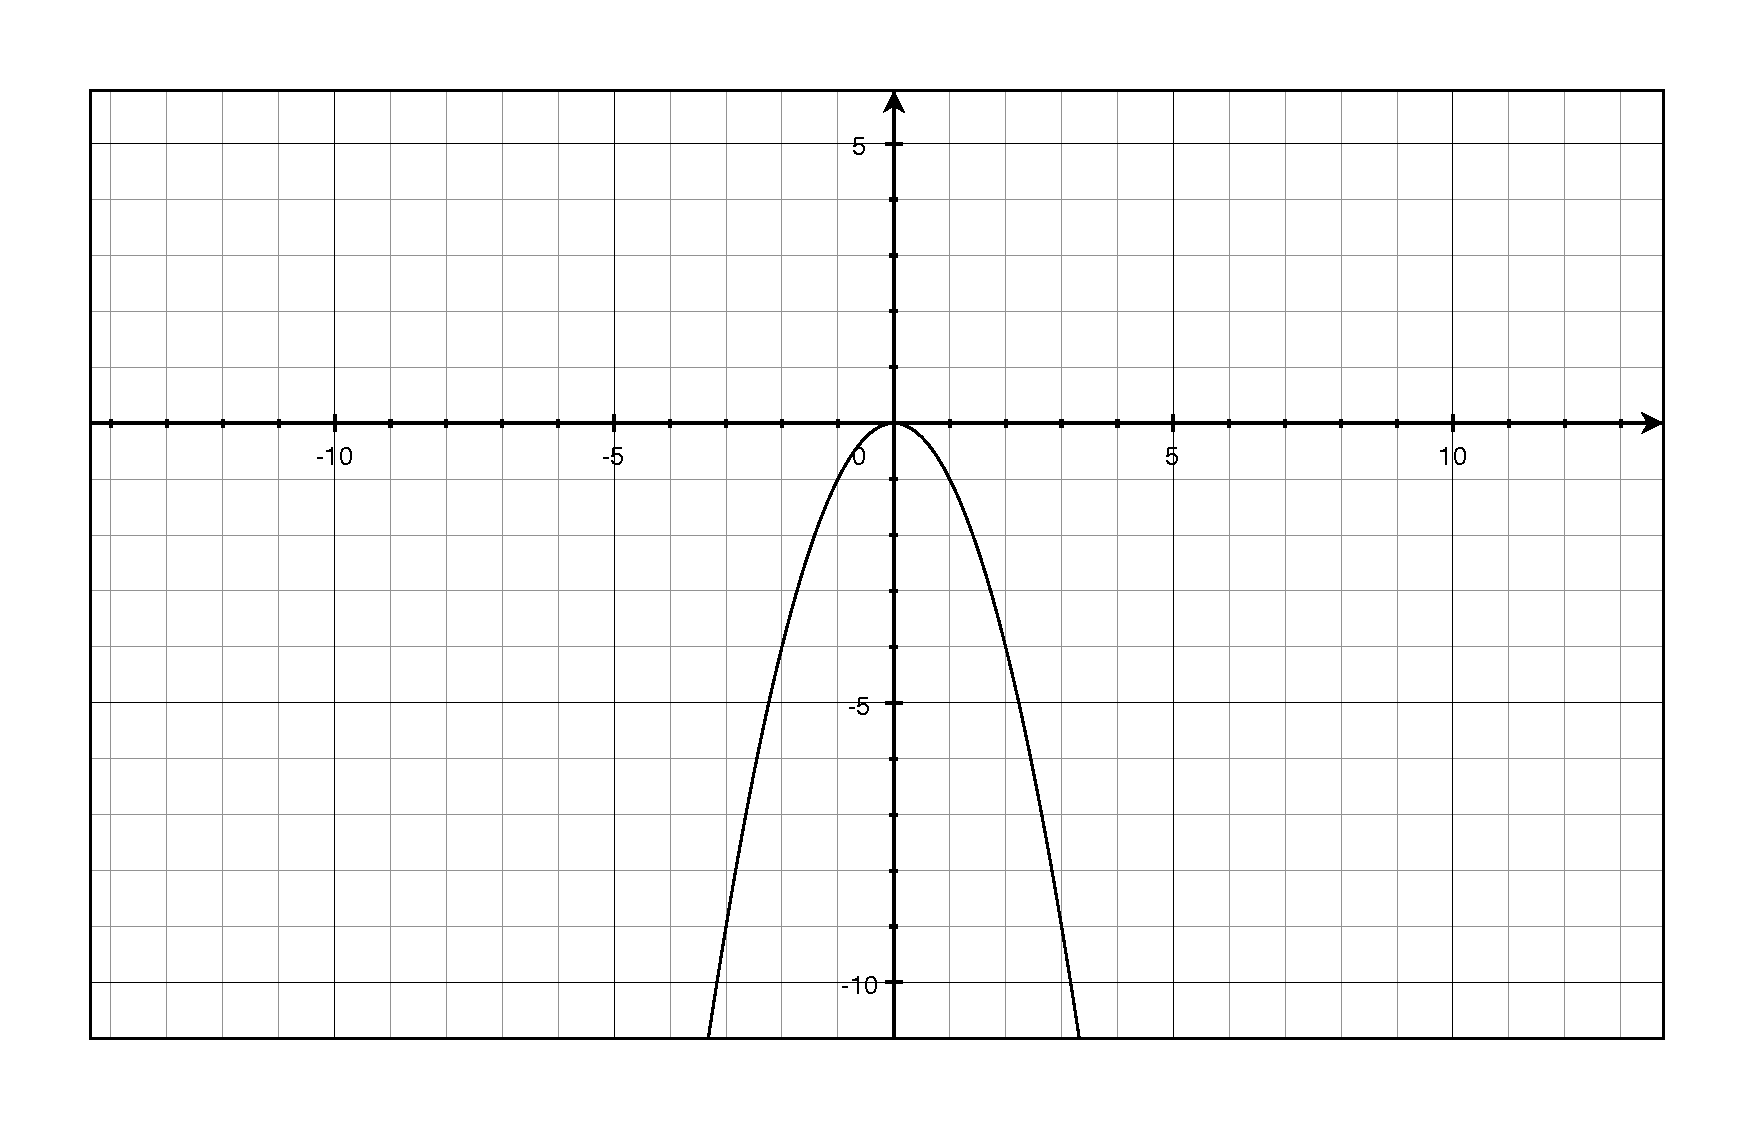
\includegraphics[scale=0.8]{problem7.eps}
%   \caption*{Problem 7}
% \end{figure}

% \begin{tabular}{cc}
%   \toprule
%   period & amplitude \\
%   \midrule
%   value one & value two
%   \bottomrule
% \end{tabular}

\printanswers

\ifprintanswers 
  \usepackage{2in1, lscape} 
\fi

\date{June 26, 2013}
\author{}
\title{Math 141 \\ Homework 16}

\begin{document}

  \maketitle

  \section{Homework}

  Section 4.4: 

  \ifprintanswers
    \pagebreak
  \fi

  \section{Extra Credit}
  Section 4.4: TO DO

  \ifprintanswers
    \begin{description}
      \item[61]
        \begin{align*}
          - \log(x - \sqrt{x^2 - 1}) &= \log(x - \sqrt{x^2 - 1})^{-1} \\
                                     &= \log \frac{1}{x - \sqrt{x^2 - 1}} \\
                                     &= \log \left[ \frac{1}{x - \sqrt{x^2 - 1}} \cdot \frac{x + \sqrt{x^2 - 1}}{x + \sqrt{x^2 - 1}} \right] \\
                                     &= \log \left[ \frac{x + \sqrt{x^2 - 1}}{x^2 - (x^2 - 1)} \right] \\
                                     &= \log ( x + \sqrt{x^2 - 1} ) \\
        \end{align*}

    \end{description}
  \fi

  \ifprintanswers
    \pagebreak
  \fi

  \section{Review}

  Graph each function
  \begin{enumerate}

    \item $f(x) = x + |x|$ 
      \ifprintanswers
        TO DO
      \fi

  \end{enumerate}

  \ifprintanswers
    \section{Section 4.4}

    \begin{description}

      \item[35] 
        \begin{align*}
          \ln x &= 10 \\
          x     &= \boxed{e^{10}} \\
        \end{align*}

      \item[36] 
        \begin{align*}
          ln (2 + x) &= 1 \\
          2 + x      &= e \\
          x          &= \boxed{e - 2} \\
        \end{align*}

      \item[37] 
        \begin{align*}
          \log x &= -2 \\
          x      &= 10^{-2} \\
                 &= \boxed{\frac{1}{100}} \\
        \end{align*}

      \item[38] 
        \begin{align*}
          \log (x - 4) &= 3 \\
          x - 4        &= 10^3 \\
          x            &= \boxed{996} \\
        \end{align*}

      \item[39] 
        \begin{align*}
          \log (3x + 5) &= 2 \\
          3x + 5        &= 10^2 \\
          x             &= \boxed{\frac{95}{3}} \\
        \end{align*}

      \item[40] 
        \begin{align*}
          \log_2 (2 - x) &= 3 \\
          2 - x          &= 2^3 \\
          x              &= \boxed{-6} \\
        \end{align*}

      \item[41] 
        \begin{align*}
          2 - \ln(3 - x) &= 0 \\
          \ln(3 - x)     &= 2 \\
          3 - x          &= e^2 \\
          x              &= \boxed{3 - e^2} \\
        \end{align*}

      \item[42] 
        \begin{align*}
          \log_2(x^2 - x - 2) &= 2 \\
          x^2 - x - 2         &= 2^2 \\
          x^2 - x - 6         &= 0 \\
          (x - 3)(x + 2)      &= 0 \\
          x                   &= \boxed{\{ - 2, 3\}} \\
        \end{align*}

      \item[43] 
        \begin{align*}
          \log_2 3 + \log_2 x &= \log_2 5 + \log_2(x - 2) \\
          \log_2 3x           &= \log_2 [5 (x - 2)] \\
          3x                  &= 5x - 10 \\
          x                   &= \boxed{5} \\
        \end{align*}

      \item[44] 
        \begin{align*}
          2 \log x       &= \log 2 + \log(3x - 4) \\
          \log x^2       &= \log [2(3x - 4)] \\
          x^2            &= 6x - 8 \\
          x^2 - 6x + 8   &= 0 \\
          (x - 4)(x - 2) &= 0 \\
          x              &= \boxed{\{2, 4\}} \\
        \end{align*}

      \item[45] 
        \begin{align*}
          \log x + \log(x - 1) &= \log (4x) \\
          \log [x(x - 1)]      &= \log (4x) \\
          x^2 - x              &= 4x \\
          x^2 - 5x             &= 0 \\
          x(x - 5)             &= 0 \\
          x                    &= \boxed{5} \\
        \end{align*}

      \item[46] 
        \begin{align*}
          \log_5 x + \log_5(x + 1) &= \log_5 20 \\
          \log_5 [x(x + 1)]        &= \log_5 20 \\
          x^2 + x                  &= 20 \\
          x^2 + x - 20             &= 0 \\
          (x + 5)(x - 4)           &= 0 \\
          x                        &= \boxed{4} \\
        \end{align*}

      \item[47] 
        \begin{align*}
          \log_5 (x + 1) - \log_5 (x - 1) &= 2 \\
          \log_5 \frac{x + 1}{x - 1}      &= 2 \\
          \frac{x + 1}{x - 1}             &= 5^2 \\
          x + 1                           &= 25x - 25 \\
          24x                             &= 26 \\
          x                               &= \boxed{\frac{13}{12}} \\
        \end{align*}

      \item[48] 
        \begin{align*}
          \log x + \log (x - 3)        &= 1 \\
          \log \left( x^2 - 3x \right) &= 1 \\
          x^2 - 3x                     &= 10 \\
          x^2 - 3x - 10                &= 0 \\
          (x - 5)(x + 2)               &= 0 \\
          x                            &= \boxed{5} \\
        \end{align*}

    \end{description}

  \else
    \vspace{5 cm}
    \begin{quote}
      \begin{em}
        TO DO
      \end{em}
    \end{quote}

    \hspace{1 cm} --Peter Kropotkin
  \fi

\end{document}

